\section{Overall Product Description}
\label{sec:overall_description}


\subsection{Product Perspective}
\label{sub:product_perspective}
% Begin SubSection
There are a multitude of applications and websites for identifying languages based on text. However, the main product to compare this product to is Google Translate, 
as it is widely used and has a built-in language detector. The main difference between the two products is that Google Translate is inherently a translator
and the language detector is a non-functional feature. On the other hand, \textbf{Languify} does not have a translator feature and functions primarily as a language identifier.
It does have the additional unique feature of providing facts about the language as a summary, which is not provided by Google Translate. \\ \\
\textbf{Languify} is not totally self-contained as it will be composed of multiple interacting systems. These components are the Expert Manager, the three \textbf{experts}, 
the Controller, Language Info, and Layout Rules. They are outlined in the block diagram below:
% End SubSection

\begin{figure}[H]
	\centering
	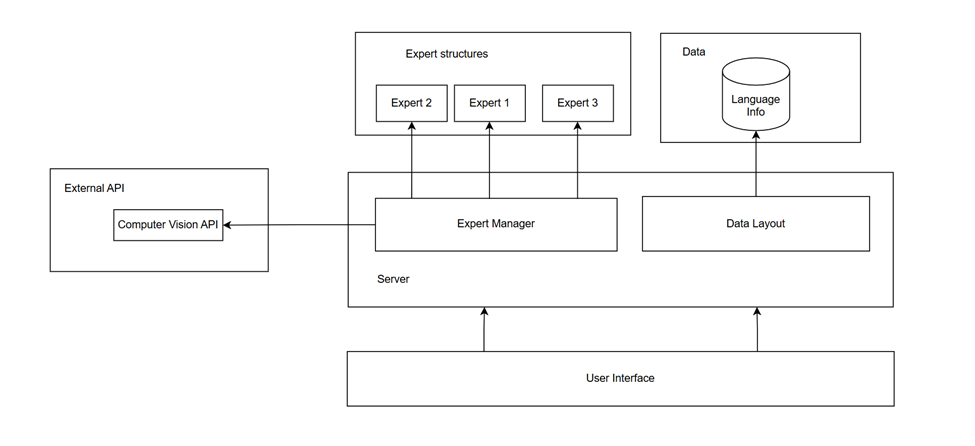
\includegraphics{Section2/Block_Diagram.png}
	\caption{Block Diagram}
	\label{BlockDiagram}
\end{figure}

\subsection{Product Functions}
\label{sub:product_functions}
% Begin SubSection
There will be three modules in the product: the Reader Service, the Identifier Service, and the Facts Service.

\begin{longtable}{p{0.5\linewidth} | p{0.5\linewidth}}
\toprule
\textbf{Modules} & \textbf{Functions} \\
\midrule
\endhead

\textbf{Reader Service} & 
\begin{itemize}
    \item \textbf{Read PDF} – Allows the user to input a PDF document that contains the language that they want to identify.
    \item \textbf{Read Text} – Allows the user to input text of the language that they want to identify.
    \item \textbf{Read Photo} – Allows the user to input a photo of the language they want to identify.
\end{itemize} \\

\hline

\textbf{Identifier Service} & 
\begin{itemize}
    \item \textbf{Identify Language} – Identifies the language that was inputted by the user.
\end{itemize} \\


\hline

\textbf{Facts Service (Innotive Feature)} & 
\begin{itemize}
    \item \textbf{List How Many Speakers} – Gives an estimate of how many speakers of the identified language in the world and displays it to the user.
    \item \textbf{Display Map} – Displays a world map highlighting the regions where the identified language is most commonly spoken.
    \item \textbf{List Phrases} – Lists common phrases in that language and how to pronounce them to the user.
    \item \textbf{Generate Facts} – Generates all the required facts about the identified language.
\end{itemize} \\
\bottomrule
\end{longtable}


\begin{figure}[H]
	\centering
	% \includegraphics[width=\linewidth]bg{Example_Use_Case.png}
	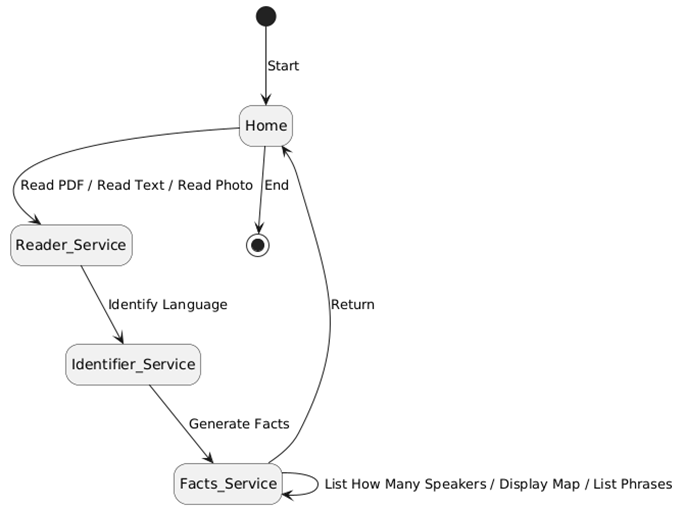
\includegraphics{Section2/State_Diagram.png}
	\caption{State Diagram}
	\label{StateDiagram}
\end{figure}
% End SubSection


\subsection{User Characteristics}
\label{sub:user_characteristics}
% Begin SubSection
\begin{itemize}
	\item \textbf{Experience with Application}: The user may range anywhere from being a first-time user to having many experiences with the application.
	\item \textbf{Experience with Technology}: The user has at least one month of experience using a smartphone and can perform basic actions such as taking photos, selecting a file for upload, and typing into a text box.
	\item \textbf{Education}: The user can read and write in English. They have a very basic knowledge about geography, world languages, and culture. 
	\item \textbf{Age}: The user is at least 13 years old but is likely an older teen or adult.
	\item \textbf{Physical Ability}:  The user may be able-bodied or disabled.
	\item \textbf{Location}: The user is likely located in a culturally diverse area, whether that is due to travel or residence.
	\item \textbf{Personality}: The user is likely curious about other cultures and languages.
\end{itemize}

% End SubSection

\subsection{Constraints}
\label{sub:constraints}
% Begin SubSectionf
\begin{itemize}
	\item \textbf{Budget}: The budget is a significant constraint on the developers' options. There are costly \textbf{API}s, design tools, and hosting infrastructure that can either significantly improve the quality of the product or streamline its development. Since this is a school project, the allotted budget is \textdollar 0, which leaves these products unavailable to developers.
	\item \textbf{Time}: The product must be completed by the end of the term, which is in just a little over 2 months. This short timeframe means that the product will have limited features and possibly limited functionality.
	\item \textbf{Platform}: The product must be a mobile application designed for Android Operating System. This constrains the developer to make an application layout that fits the dimensions of smartphones. The functions of the application must be limited to ones that are available for the Android Operating System and mobile devices. Finally, the size of the application must fit within the phone's memory.
\end{itemize}

% End SubSection

\subsection{Assumptions and Dependencies}
\label{sub:assumptions_and_dependencies}
% Begin SubSection
\begin{itemize}
	\item Assumes that the language being identified exists.
	\item Assumes that the user using the application has basic technology experience.
	\item Assumes that the input from the user is legible and clear.
	\item Assumes that the user has a smartphone with a functioning camera.
	\item Assumes that the user has an up-to-date operating system to run the application.
	\item Assumes that the user is satisfied with the application identifying a broader language category and not a specific dialect of a language.
	\item Assumes that the \textbf{API}s are fully functional when the application is in operation.
	\item Assumes that the \textbf{API}s are safe and secure to use.
\end{itemize}
% End SubSection




\subsection{Apportioning of Requirements}
\label{sub:apportioning_of_requirements}
% Begin SubSection
\begin{itemize}
	\item Further Language Support
	\begin{itemize}
		\item The application will only be developed in English for the first version of the application.
	\end{itemize}
	\item Further Language Identification
	\begin{itemize}
		\item In future versions, the application will be able to identify more languages with over 100 speakers.
	\end{itemize}
	\item Translator Feature
	\begin{itemize}
		\item In future versions, the application will incorporate a translator feature to be able to not only identify what the language is but translate what it is saying as well.
	\end{itemize}
\end{itemize}
% End SubSection

% End Section